\documentclass[Rapport/Rapport_main.tex]{subfiles}
\begin{document}
\subsection{Development View}
Formålet med dette view er at få overblik over hele applikation. Her illustreres de forskellige lag for applikation og tilhørende moduler og deres forbindelser. Figur \ref{fig:PackageDiagram} viser et Model Package diagram, som viser koblingerne mellem lagene og de interne komponenter. 
\begin{figure}[H]
    \centering
    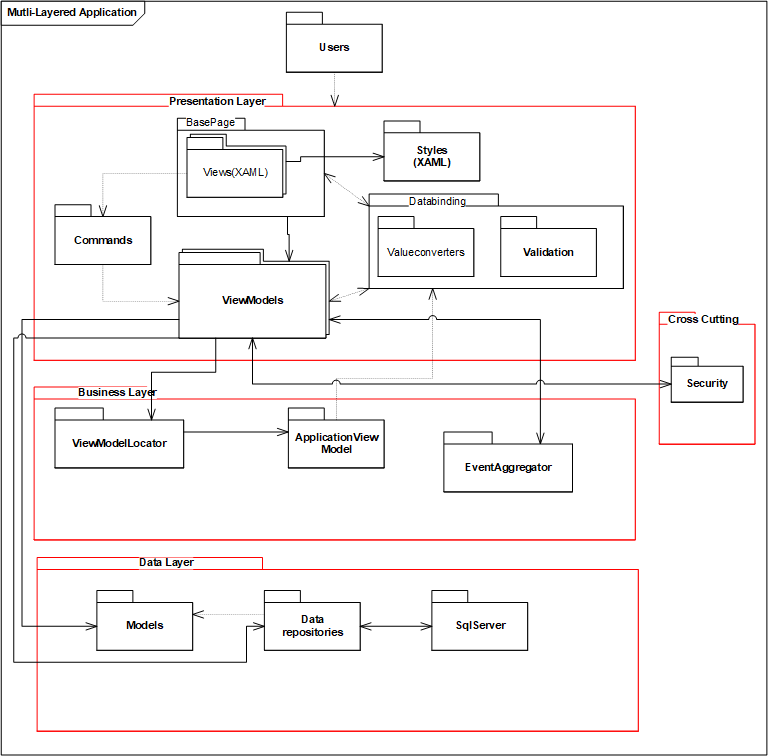
\includegraphics[width=\textwidth]{Arkitektur/4+1View/Graphics/PackageDiagram.png}
    \caption{Model diagram for Multi-Layered Applikation. En stiplet linje indikerer en forbindelse, som skabes gennem WPF frameworket - eksempelvis databinding}
    \label{fig:PackageDiagram}
\end{figure}
\end{document}